\begin{figure}[t]
%  \begin{minipage}[H]{0.45\linewidth}
%\captionsetup[subfigure]{font={bf,large}, skip=1pt, margin=-0.7cm,justification=raggedright, singlelinecheck=false}
\hfill
\centering
\begin{subcaptionblock}{0.6\linewidth}
\centering
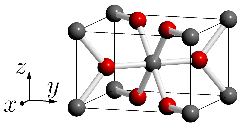
\includegraphics[]{figures/crystal_structure/rutile_axis-1_0.pdf}
\subcaption{}
\end{subcaptionblock}\hfill
\begin{subcaptionblock}{0.4\linewidth}
\centering
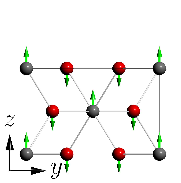
\includegraphics[width=\linewidth]{figures/A2u/A2u.pdf}
\subcaption{$A_{\mathrm{2u}}$}
\end{subcaptionblock}\hfill
\begin{subcaptionblock}{0.3\linewidth}
\centering
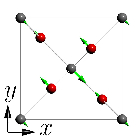
\includegraphics[width=\linewidth]{figures/E1u/E1u.pdf}
\subcaption{$E^{1}_{\mathrm{u}}$}
\end{subcaptionblock}\hfill
\begin{subcaptionblock}{0.3\linewidth}
\centering
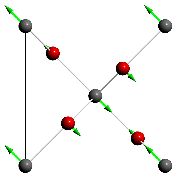
\includegraphics[width=\linewidth]{figures/E2u/E2u.pdf}
\subcaption{$E^{2}_{\mathrm{u}}$}
\end{subcaptionblock}\hfill
\begin{subcaptionblock}{0.3\linewidth}
\centering
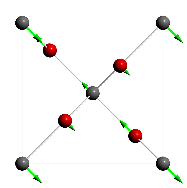
\includegraphics[width=\linewidth]{figures/E3u/E3u.pdf}
\subcaption{$E^{3}_{\mathrm{u}}$}
\end{subcaptionblock}\hfill
% \subfloat[][]{%\label{fig:modes}
%\begin{tabular}[b]{@{}c@{}}
%\end{tabular}%
%}
\caption{(a) The unit cell of rutile \ce{TiO2}, which contains two titanium atoms (black) and four oxygen atoms (red). (b-e) Schematic views of atomic displacements for the $A_{\mathrm{2u}}$ mode and the three $E_{\mathrm{u}}$ modes. }
% BZありversion \caption{(a)The crystal structure of rutile \ce{TiO2}, (b) The first Brillouin zone and its high-symmetry points including $Z (0,0,0.5)$ (reduced coordinates), $A (0.5,0.5,0.5)$, $M (0.5,0.5,0)$, $R (0,0.5,0.5)$, and $X (0,0.5,0)$, and (c) schematic view of the A_{\mathrm{2u}} mode(left) and the Eu mode(right). }
\label{fig:crystal}
\end{figure}